\documentclass[14pt]{extarticle}
\usepackage{fontspec}
\usepackage{polyglossia}
\usepackage{amsmath}
\usepackage{amssymb}
\usepackage{xcolor}
\usepackage{fancyhdr}
\usepackage{graphicx}
\usepackage{listings}
\usepackage[most]{tcolorbox}
% \usepackage{setspace}
\usepackage{pifont}
\usepackage{enumitem}
\usepackage{titlesec}
\usepackage[bottom]{footmisc}
\usepackage{titling}
\usepackage{minted}
\usepackage{etoolbox}
\usepackage{array}
\usepackage{extsizes}
\usepackage{float}
\usepackage{booktabs}
\usepackage{hyperref}
\usepackage[onehalfspacing]{setspace}
\usepackage[a4paper, top=2.7cm, bottom=2.7cm, left=2.5cm, right=2.5cm, headheight=1.5cm, headsep=0.5cm]{geometry}
\usepackage{tikz}

\usetikzlibrary{automata, positioning, arrows.meta, arrows}

\newfontfamily\emoji{Segoe UI Emoji}

\pagestyle{fancy}

\setmainlanguage[numerals=western]{arabic}
\setotherlanguage{english}
% \newfontfamily\arabicfont[Script=Arabic]{Amiri}
\newfontfamily\arabicfont[Script=Arabic]{Calibri}
\newfontfamily\arabicfonttt[Script=Arabic]{Courier New}

\lstset{
  language=[Sharp]C,
  numbers=left,
  stepnumber=1,
  numbersep=8pt,
  frame=single,
  basicstyle=\ttfamily\small,
  keywordstyle=\color{blue},
  stringstyle=\color{red},
  commentstyle=\color{green!50!black}
}

\newif\ifdetailed
\ifdefined\setdetailed
  \setdetailed
\fi

\newif\ifwithsols
\ifdefined\setwithsols
  \setwithsols
\fi

% unified tcolorboxes for articles
\tcbset{colback=white, colframe=black, fonttitle=\bfseries, boxrule=0.8pt}
\newtcolorbox{boxDef}[1][]{colback=blue!5!white,colframe=blue!75!black,
  title={{\emoji📘} تعريف\ifx\\#1\\\else ~#1\fi :}}
\newtcolorbox{boxExercise}[1][]{colback=cyan!5!white,colframe=cyan!70!black,
  title={{\emoji🧩} تمرين\ifx\\#1\\\else ~#1\fi :}}
\newtcolorbox{boxExample}[1][]{colback=yellow!5!white,colframe=orange!90!black,
  title={{\emoji📝} مثال\ifx\\#1\\\else ~#1\fi :}}
\newtcolorbox{boxNote}[1][]{colback=gray!10!white,colframe=black,
  title={{\emoji✨} ملاحظة\ifx\\#1\\\else ~#1\fi :}}
\newtcolorbox{boxAttention}[1][]{colback=magenta!10!white,colframe=magenta!80!black,
  title={{\emoji🔔} تنبيه\ifx\\#1\\\else ~#1\fi :}}
\newtcolorbox{boxWarning}[1][]{colback=red!5!white,colframe=red!75!black,
  title={{\emoji⚡} ملاحظة هامة\ifx\\#1\\\else ~#1\fi :}}
\newtcolorbox{boxSolution}[1][]{colback=green!5!white,colframe=green!60!black,
  title={{\emoji✅} حل\ifx\\#1\\\else ~#1\fi :}}
\newtcolorbox{boxSymbol}[1][]{colback=purple!5!white,colframe=purple!70!black,
  title={{\emoji🔣} رمز\ifx\\#1\\\else ~#1\fi :}}
\newtcolorbox{boxHint}[1][]{colback=teal!5!white,colframe=teal!60!black,
  title={{\emoji💡} تلميح\ifx\\#1\\\else ~#1\fi :}}


\tcbset{simplecode/.style={ colback=gray!5, colframe=black!50, boxrule=0.4pt, arc=2pt, left=4pt,right=4pt,top=4pt,bottom=4pt}}
\newenvironment{boxCode}{\begin{tcolorbox}[simplecode]}{\end{tcolorbox}}

\newcolumntype{C}[1]{>{\centering\arraybackslash}p{#1}}

% redefine spaces after titles
\makeatletter
\renewcommand{\@maketitle}{%
  \begin{center}
    {\huge \bfseries \@title \par}%
    \vskip 0.2em % space between title and author
    {\large \@author \par}%
    % \vskip 0.2em % space between author and date
    % {\normalsize \@date \par}%
  \end{center}
}
\makeatother

\fancyhf{} % clear default
\fancypagestyle{plain}{
  \fancyhf{}
  \fancyhead[L]{مدرسة التسامح الشاملة}
  % \fancyhead[L]{
\includegraphics[height=1cm]{../../../images/logoTasamoh.png}}
  \fancyhead[R]{الأستاذ محمود اغبارية}
  \fancyfoot[C]{\thepage}
}

\fancyhead[L]{مدرسة التسامح الشاملة}
\fancyhead[R]{الأستاذ محمود اغبارية}
\fancyfoot[C]{\thepage}
% \date{\today}

\setcounter{tocdepth}{3} % only section subsection and subsubsection in TOC

\newcommand{\importpdfpage}[2]{%
    \thispagestyle{empty}
    \newgeometry{left=0cm,right=0cm,top=0cm,bottom=0cm}
    \includegraphics[page=#2,width=0.95\paperwidth,height=0.95\paperheight,keepaspectratio]{#1}
    \restoregeometry
}

\newcommand{\insertFullImg}[1]{%
    \noindent
    \makebox[\textwidth][c]{
        \includegraphics[width=0.9\paperwidth,keepaspectratio]{#1}%
    }%
}%

% ----------------------


% \begin{document}

% \maketitle

% % \clearpage  % start TOC on a new page
% % \renewcommand{\contentsname}{جدول المحتويات}
% % \tableofcontents
% % \clearpage

% \part*{part 1} % the * prevents numbering
% \section*{مقدمة}
% \subsection*{مثال رياضي}
% \subsubsection*{مثال فرعي}
% \paragraph*{ paragraph 1}
% \subparagraph*{sub paragraph 1}

% \ifdetailed
% \begin{english}
% \begin{minted}{csharp}
% // C# Example
% \end{minted}
% \end{english}
% \fi

% OLD WAY
% \ifdetailed
% \begin{english}
% \begin{lstlisting}
% // C# Example
% \end{lstlisting}
% \end{english}
% \fi

% % 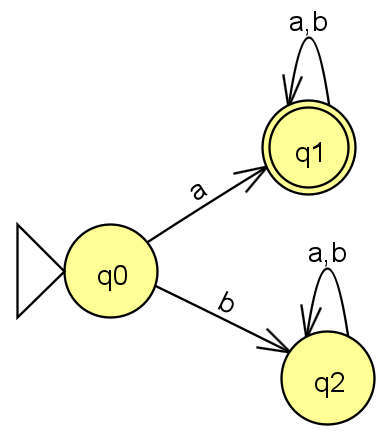
\includegraphics[width=0.2\textwidth]{../../../images/DFAs/ex1_q1.png}



% \vspace{3cm}
% \begin{flushleft}
% أرجو لكم وقتًا ممتعًا.

% الأستاذ محمود اغبارية.
% \end{flushleft}


% \end{document}


\title{ورقة تمرّن شاملة: الفئات والكائنات المتقدّمة}

\begin{document}

\maketitle
\thispagestyle{fancy}

%=============================================================
\section{فئة تحتوي على خاصية من نوع فئة أخرى}
%=============================================================

تستخدم هذه الأسئلة الفئتين \textenglish{Department} و\textenglish{Employee}:

\begin{boxExample}
\begin{english}
{\small
\begin{minted}{csharp}
class Department
{
    private string Name;
    private int    Floor;

    public Department(string name, int floor)
    {
        this.Name  = name;
        this.Floor = floor;
    }
    public string GetName()  { return Name;  }
    public int    GetFloor() { return Floor; }
    public void Print()
    {
        Console.WriteLine($"Dept: {Name}, Floor {Floor}");
    }
}

class Employee
{
    private string     Name;
    private double     Salary;
    private Department Dept;

    public Employee(string name, double salary, Department dept)
    {
        this.Name   = name;
        this.Salary = salary;
        this.Dept   = dept;
    }
    public string     GetName()   { return Name;   }
    public double     GetSalary() { return Salary; }
    public Department GetDept()   { return Dept;   }
    public void SetSalary(double s) { if (s > 0) Salary = s; }
    public void Print()
    {
        Console.WriteLine(
            $"{Name} | Salary: {Salary} | {Dept.GetName()}");
    }
}
\end{minted}
}
\end{english}
\end{boxExample}

\begin{enumerate}

%--- سؤال 3.1 ---
\item
أنشئ في \textenglish{Main} قسمًا (\textenglish{Department}) وموظفَين يعملان فيه،
ثم اطبع كل موظف:

\begin{center}
\begin{tabular}{|c|c|c|}
\hline
\textbf{الموظف} & \textbf{الراتب} & \textbf{القسم / الطابق} \\
\hline
\textenglish{Hana}  & \textenglish{8000} & \textenglish{HR, Floor 2} \\
\textenglish{Tariq} & \textenglish{9500} & \textenglish{HR, Floor 2} \\
\hline
\end{tabular}
\end{center}

\ifwithsols
\textbf{الشرح:}
\begin{english}
{\small
\begin{minted}{csharp}
// In Main
Department hr = new Department("HR", 2);

Employee e1 = new Employee("Hana",  8000, hr);
Employee e2 = new Employee("Tariq", 9500, hr);

e1.Print();
e2.Print();
\end{minted}
}
\end{english}
\clearpage
\fi

%--- سؤال 3.2 ---
\item
بافتراض وجود \textenglish{e1} و\textenglish{e2} من السؤال السابق،
اكتب كودًا يطبع اسم القسم الذي يعمل فيه \textenglish{e1} ورقم طابقه.

\ifwithsols
\textbf{الشرح:}
\begin{english}
{\small
\begin{minted}{csharp}
// In Main
Console.WriteLine("Department: " + e1.GetDept().GetName());
Console.WriteLine("Floor: " + e1.GetDept().GetFloor());
\end{minted}
}
\end{english}
\clearpage
\fi

%--- سؤال 3.3 ---
\item
أضِف إلى الفئة \textenglish{Employee} عملية \textenglish{IsInSameDept(Employee other)}
تُعيد \textenglish{true} إذا كان الموظفان في نفس القسم (نفس اسم القسم).

اختبِرها في \textenglish{Main}.

\ifwithsols
\textbf{الشرح:}
\begin{english}
{\small
\begin{minted}{csharp}
// Inside class Employee
public bool IsInSameDept(Employee other)
{
    return this.Dept.GetName() == other.Dept.GetName();
}

// In Main
if (e1.IsInSameDept(e2))
    Console.WriteLine("Same department.");
else
    Console.WriteLine("Different departments.");
\end{minted}
}
\end{english}
\clearpage
\fi

%--- سؤال 3.4 ---
\item
أنشئ في \textenglish{Main} موظفَين من قسمَين مختلفَين:

\begin{center}
\begin{tabular}{|c|c|c|}
\hline
\textbf{الموظف} & \textbf{الراتب} & \textbf{القسم / الطابق} \\
\hline
\textenglish{Mona}  & \textenglish{7200} & \textenglish{Sales, Floor 1} \\
\textenglish{Ziad}  & \textenglish{8800} & \textenglish{IT, Floor 3} \\
\hline
\end{tabular}
\end{center}

ثم اكتب كودًا يطبع اسم الموظف الأعلى راتبًا واسم قسمه.

\ifwithsols
\textbf{الشرح:}
\begin{english}
{\small
\begin{minted}{csharp}
// In Main
Department sales = new Department("Sales", 1);
Department it    = new Department("IT", 3);

Employee m1 = new Employee("Mona", 7200, sales);
Employee m2 = new Employee("Ziad", 8800, it);

Employee higher = (m1.GetSalary() > m2.GetSalary()) ? m1 : m2;
Console.WriteLine(higher.GetName()
    + " - " + higher.GetDept().GetName());
\end{minted}
}
\end{english}
\clearpage
\fi

%--- سؤال 3.5 ---
\item
أضِف إلى الفئة \textenglish{Employee} عملية بنّاءة ثانية تتلقى الاسم والراتب فقط،
وتُهيّئ \textenglish{Dept} بكائن افتراضي اسمه \textenglish{"Unassigned"} وطابقه \textenglish{0}.

أضِف أيضًا عملية \textenglish{SetDept(Department d)} تسمح بتعيين القسم لاحقًا.

اختبِرها في \textenglish{Main} بإنشاء موظف بدون قسم، ثم تعيين قسم له وطباعته.

\ifwithsols
\textbf{الشرح:}
\begin{english}
{\small
\begin{minted}{csharp}
// Inside class Employee — second constructor
public Employee(string name, double salary)
{
    this.Name   = name;
    this.Salary = salary;
    this.Dept   = new Department("Unassigned", 0);
}

// Inside class Employee — SetDept
public void SetDept(Department d)
{
    if (d != null)
        this.Dept = d;
}

// In Main
Employee e3 = new Employee("Layla", 7500);
e3.Print(); // Layla | Salary: 7500 | Unassigned

Department dev = new Department("Development", 4);
e3.SetDept(dev);
e3.Print(); // Layla | Salary: 7500 | Development
\end{minted}
}
\end{english}
\fi

\end{enumerate}

\clearpage
%=============================================================
\section{فئة تحتوي على مصفوفة كائنات من فئة أخرى}
%=============================================================

تستخدم هذه الأسئلة الفئتين \textenglish{Product} و\textenglish{Store}:

\begin{boxExample}
\begin{english}
{\small
\begin{minted}{csharp}
class Product
{
    private string Name;
    private double Price;
    private int    Stock; // quantity in storage

    public Product(string name, double price, int stock)
    {
        this.Name  = name;
        this.Price = price;
        this.Stock = stock;
    }
    public string GetName()  { return Name;  }
    public double GetPrice() { return Price; }
    public int    GetStock() { return Stock; }
    public bool IsAvailable() { return Stock > 0; }
    public void Print()
    {
        Console.WriteLine($"{Name} | {Price} NIS | Stock: {Stock}");
    }
}

class Store
{
    private string    Name;
    private Product[] Products;

    public Store(string name, Product[] products)
    {
        this.Name     = name;
        this.Products = products;
    }
    public string    GetName()     { return Name;     }
    public Product[] GetProducts() { return Products; }
    public void PrintAll()
    {
        Console.WriteLine($"=== {Name} ===");
        for (int i = 0; i < Products.Length; i++)
            Products[i].Print();
    }
}
\end{minted}
}
\end{english}
\end{boxExample}

\begin{enumerate}

%--- سؤال 4.1 ---
\item
أنشئ في \textenglish{Main} مصفوفة منتجات \textenglish{products} بالبيانات التالية،
ثم أنشئ متجرًا باسم \textenglish{"Tech Shop"} وملئه بها، واطبع جميع منتجاته:

\begin{center}
\begin{tabular}{|c|c|c|}
\hline
\textbf{المنتج} & \textbf{السعر} & \textbf{الكمية} \\
\hline
\textenglish{Keyboard} & \textenglish{120} & \textenglish{5} \\
\textenglish{Mouse}    & \textenglish{80}  & \textenglish{0} \\
\textenglish{Monitor}  & \textenglish{950} & \textenglish{3} \\
\hline
\end{tabular}
\end{center}

\ifwithsols
\textbf{الشرح:}
\begin{english}
{\small
\begin{minted}{csharp}
// In Main
Product[] products = new Product[3];
products[0] = new Product("Keyboard", 120, 5);
products[1] = new Product("Mouse",    80,  0);
products[2] = new Product("Monitor",  950, 3);

Store store = new Store("Tech Shop", products);
store.PrintAll();
\end{minted}
}
\end{english}
\clearpage
\fi

%--- سؤال 4.2 ---
\item
أضِف إلى الفئة \textenglish{Store} عملية \textenglish{CountAvailable()} تُعيد عدد
المنتجات المتوفرة في المخزن (\textenglish{Stock > 0}).

اطبع النتيجة في \textenglish{Main}.

\ifwithsols
\textbf{الشرح:}
\begin{english}
{\small
\begin{minted}{csharp}
// Inside class Store
public int CountAvailable()
{
    int count = 0;
    for (int i = 0; i < Products.Length; i++)
        if (Products[i].IsAvailable())
            count++;
    return count;
}

// In Main
Console.WriteLine("Available products: " + store.CountAvailable());
\end{minted}
}
\end{english}
\clearpage
\fi

%--- سؤال 4.3 ---
\item
أضِف إلى الفئة \textenglish{Store} عملية \textenglish{GetTotalValue()} تُعيد
القيمة الإجمالية للمخزن (\textenglish{Price * Stock} لكل منتج).

اطبع النتيجة في \textenglish{Main}.

\ifwithsols
\textbf{الشرح:}
\begin{english}
{\small
\begin{minted}{csharp}
// Inside class Store
public double GetTotalValue()
{
    double total = 0;
    for (int i = 0; i < Products.Length; i++)
        total += Products[i].GetPrice() * Products[i].GetStock();
    return total;
}

// In Main
Console.WriteLine("Store value: " + store.GetTotalValue() + " NIS");
\end{minted}
}
\end{english}
\clearpage
\fi

%--- سؤال 4.4 ---
\item
أضِف إلى الفئة \textenglish{Store} عملية \textenglish{FindMostExpensive()}
تُعيد المنتج الأغلى سعرًا في المتجر.

اطبع المنتج المُعاد في \textenglish{Main}.

\ifwithsols
\textbf{الشرح:}
\begin{english}
{\small
\begin{minted}{csharp}
// Inside class Store
public Product FindMostExpensive()
{
    Product result = Products[0];
    for (int i = 1; i < Products.Length; i++)
        if (Products[i].GetPrice() > result.GetPrice())
            result = Products[i];
    return result;
}

// In Main
Product top = store.FindMostExpensive();
Console.Write("Most expensive: ");
top.Print();
\end{minted}
}
\end{english}
\clearpage
\fi

%--- سؤال 4.5 ---
\item
أضِف إلى الفئة \textenglish{Store} عملية \textenglish{GetAvailableProducts()}
تُعيد مصفوفة جديدة تحتوي فقط المنتجات المتوفرة في المخزن.

اطبع المصفوفة المُعادة في \textenglish{Main}.

\ifwithsols
\textbf{الشرح:}
\begin{english}
{\small
\begin{minted}{csharp}
// Inside class Store
public Product[] GetAvailableProducts()
{
    int count = 0;
    for (int i = 0; i < Products.Length; i++)
        if (Products[i].IsAvailable())
            count++;

    Product[] result = new Product[count];
    int j = 0;
    for (int i = 0; i < Products.Length; i++)
    {
        if (Products[i].IsAvailable())
        {
            result[j] = Products[i];
            j++;
        }
    }
    return result;
}

// In Main
Product[] available = store.GetAvailableProducts();
Console.WriteLine("Available:");
for (int i = 0; i < available.Length; i++)
    available[i].Print();
\end{minted}
}
\end{english}
\clearpage
\fi

\end{enumerate}

\vspace{1em}
\begin{flushleft}
أرجو لكم عملاً ممتعاً!

الأستاذ محمود اغبارية
\end{flushleft}

\end{document}
